\chapter{रोज़मर्रा के जीवन में ऊर्जा}\label{ch:g5:everyday-energy}

चाबी वाला खिलौना फ़र्श पर दौड़ता है, धीमा पड़ता है, और रुक जाता है ---
जब तक तुम उसे फिर चाबी न दो। \omterm{def:g3:first-electric-circuit:battery}{बैटरी} थकते ही टॉर्च मंद पड़ जाती है। और
तुम ख़ुद दोपहर के खाने से पहले ही हाँफने लगते हो। जो भी चीज़ चलती है,
चमकती है, बजती है या गरम करती है, वह कुछ न कुछ ख़र्च करती लगती है।
भौतिकी ने उस ``कुछ'' को एक नाम दिया है, और शायद वह इस पूरी पुस्तक का
सबसे ज़रूरी शब्द है: \omterm{def:g5:everyday-energy:energy}{ऊर्जा}।

\section{वह चीज़ जो काम करवाती है}

\begin{definition}[ऊर्जा]\label{def:g5:everyday-energy:energy}
\emph{ऊर्जा}\index{ऊर्जा} वही है जो कुछ भी होने के लिए चाहिए: चीज़ों
को चलाने के लिए, उठाने के लिए, जलाने के लिए, गरम करने के लिए, और
बजाने के लिए। कुछ भी न चलता है, न चमकता है, न बढ़ता है, जब तक उस पर
ऊर्जा ख़र्च न हो --- और जो ख़र्च कर रहा है, उसके पास ख़र्च करने को
ऊर्जा पहले से होनी चाहिए।
\end{definition}

\begin{definition}[ऊर्जा भंडार]\label{def:g5:everyday-energy:store}
\emph{ऊर्जा भंडार}\index{ऊर्जा भंडार} वह हर चीज़ है जो \omterm{def:g5:everyday-energy:energy}{ऊर्जा} को काम
में आने के लिए तैयार रखती है। रोज़मर्रा के बड़े भंडार:
\emph{भोजन} (तुम्हारे शरीर का ईंधन), लकड़ी और पेट्रोल जैसे
\emph{ईंधन}, भरी हुई \emph{बैटरियाँ}, चाबी दी हुई \emph{स्प्रिंग},
बाँध के पीछे \emph{ऊँचाई} पर रुका पानी --- और गरम \emph{सूर्य}, जो
हर चीज़ पर दिन भर, मुफ़्त, \omterm{def:g5:everyday-energy:energy}{ऊर्जा} उँडेलता रहता है।
\end{definition}

\begin{example}[भंडार पहचानो]\label{ex:g5:everyday-energy:spot}
हर चलती चीज़ के पीछे कोई भंडार होता है। दौड़ता खिलौना: उसकी चाबी दी
हुई स्प्रिंग। टॉर्च: उसकी बैटरियाँ। गाड़ी: टंकी का ईंधन। तुम:
तुम्हारा नाश्ता। पालवाली नाव: \omterm{def:g2:air-around-us:wind}{पवन} की चलती \omterm{def:g2:air-around-us:air}{हवा}। भंडार ख़ाली होते ही
--- स्प्रिंग खुल गई, बैटरियाँ चुक गईं, टंकी सूख गई, दोपहर का खाना
पास आ गया --- चलना रुक जाता है।
\end{example}

\begin{remark}[खिलाओ नहीं, तो चलेगा नहीं]\label{rem:g5:everyday-energy:nofree}
सदियों तक आविष्कारक ऐसी मशीनों के पीछे भागते रहे जो बिना कुछ लिए
हमेशा चलती रहें --- ख़ुद घूमने वाले पहिये, कभी चाबी न माँगने वाली
घड़ियाँ। हर एक नाकाम रही। उनकी नाकामी भौतिकी के सबसे गहरे सबक़ों में
से एक है: \omterm{def:g5:everyday-energy:energy}{ऊर्जा} कभी \omterm{def:g2:air-around-us:air}{हवा} में से नहीं गढ़ी जाती। जो भी चल रहा है, उसे
खिलाया जा रहा है --- भंडार ढूँढ़ लो, और मशीन समझ में आ जाएगी।
\end{remark}

\section{ऊर्जा रूप बदलती है}

\begin{example}[ऊर्जा के रूप]\label{ex:g5:everyday-energy:forms}
\omterm{def:g5:everyday-energy:energy}{ऊर्जा} अलग-अलग रूपों में सामने आती है: लुढ़कती गेंद और बहती \omterm{def:g2:air-around-us:wind}{पवन} में
\emph{गति} की \omterm{def:g5:everyday-energy:energy}{ऊर्जा}; लैंप और सूर्य से उँडेलती \emph{\omterm{def:g1:light-and-shadows:source}{प्रकाश}} \omterm{def:g5:everyday-energy:energy}{ऊर्जा}; हर
गरम चीज़ में \emph{ऊष्मा} \omterm{def:g5:everyday-energy:energy}{ऊर्जा}; तारों में सफ़र करती \emph{विद्युत}
\omterm{def:g5:everyday-energy:energy}{ऊर्जा}; और भोजन, ईंधन, स्प्रिंगों तथा ऊपर उठाई गई चीज़ों में चुपचाप
इंतज़ार करती \emph{संचित} \omterm{def:g5:everyday-energy:energy}{ऊर्जा}। वही एक चीज़, अनेक रूप।
\end{example}

\begin{proposition}[ऊर्जा की शृंखला]\label{prop:g5:everyday-energy:chain}
जब भी कुछ होता है, \omterm{def:g5:everyday-energy:energy}{ऊर्जा} किसी भंडार से निकाली जाती है और आगे बढ़ा दी
जाती है, और अकसर रास्ते में अपना रूप बदल लेती है। वह न कभी शून्य से
बनाई जाती है --- और न सचमुच नष्ट होती है: मशीन जिसे ``ख़र्च कर देती
है'' वह असल में आगे बढ़ा दी गई होती है, और देर-सबेर ज़्यादातर आस-पास
में फैली हल्की गरमी बनकर ख़त्म होती है।
\end{proposition}

\begin{method}[ऊर्जा की शृंखला पढ़ना]\label{met:g5:everyday-energy:read}
किसी भी यंत्र को समझने के लिए उसकी शृंखला का पीछा करो:
\begin{enumerate}
  \item वह \emph{भंडार} ढूँढ़ो जहाँ से \omterm{def:g5:everyday-energy:energy}{ऊर्जा} आती है;
  \item वह \emph{रूपांतरक} ढूँढ़ो --- यानी वह हिस्सा जहाँ \omterm{def:g5:everyday-energy:energy}{ऊर्जा} अपना
        रूप बदलती है;
  \item बाहर निकलने वाले रूपों के नाम बताओ --- काम का रूप, और उसके
        साथ रिसने वाली गरमी।
\end{enumerate}
टॉर्च का पीछा करने पर: \omterm{def:g3:first-electric-circuit:battery}{बैटरी} (भंडार) $\to$ \omterm{def:g3:first-electric-circuit:bulb}{बल्ब} (रूपांतरक) $\to$
\omterm{def:g1:light-and-shadows:source}{प्रकाश} (काम का) $+$ थोड़ी गरमी (रिसाव --- \omterm{def:g3:first-electric-circuit:bulb}{बल्ब} छूकर देखो)।
\end{method}

\begin{omfigure}
\begin{tikzpicture}[scale=0.85]
  \node[draw, thick, omDef, font=\small, minimum width=2.5cm,
    minimum height=0.9cm] (a) at (1.4,0) {बैटरी: भंडार};
  \node[draw, thick, omMeth, font=\small, minimum width=2.5cm,
    minimum height=0.9cm] (b) at (5.4,0) {बल्ब: रूपांतरक};
  \node[draw, thick, omThm, font=\small, minimum width=2.2cm,
    minimum height=0.9cm] (c) at (9.4,0.7) {प्रकाश: काम का};
  \node[draw, thick, omExo, font=\small, minimum width=2.2cm,
    minimum height=0.9cm] (d) at (9.4,-0.7) {गरमी: रिसाव};
  \draw[-Stealth, very thick] (a) -- (b);
  \draw[-Stealth, very thick] (b) -- (c);
  \draw[-Stealth, very thick] (b) -- (d);
\end{tikzpicture}

{\small टॉर्च की \omterm{def:g5:everyday-energy:energy}{ऊर्जा} शृंखला: संचित \omterm{def:g5:everyday-energy:energy}{ऊर्जा} \omterm{def:g1:light-and-shadows:source}{प्रकाश} बन जाती है ---
और साथ में थोड़ी गरमी हमेशा फिसलकर निकल जाती है।}
\end{omfigure}

\begin{example}[हर जगह शृंखलाएँ]\label{ex:g5:everyday-energy:chains}
तुम्हारी सुबह की साइकिल-सवारी का पीछा: नाश्ता (भंडार) $\to$ तुम्हारी
माँसपेशियाँ (रूपांतरक) $\to$ साइकिल की गति $+$ गरमी (तुम्हें महसूस
होती है --- तुम तप उठते हो)। पवन-खेत: चलती \omterm{def:g2:air-around-us:air}{हवा} $\to$ घूमते पंख $\to$
तारों में विद्युत \omterm{def:g5:everyday-energy:energy}{ऊर्जा} $\to$ आज रात तुम्हारे लैंप का \omterm{def:g1:light-and-shadows:source}{प्रकाश}। बाँध:
ऊँचाई का पानी $\to$ गिरता पानी टरबाइन घुमाता है $\to$ विद्युत \omterm{def:g5:everyday-energy:energy}{ऊर्जा}।
लंबी शृंखलाएँ छोटी शृंखलाओं को जोड़कर ही बनती हैं: रूप के बाद रूप,
और फिर रूप।
\end{example}

\begin{omfigure}
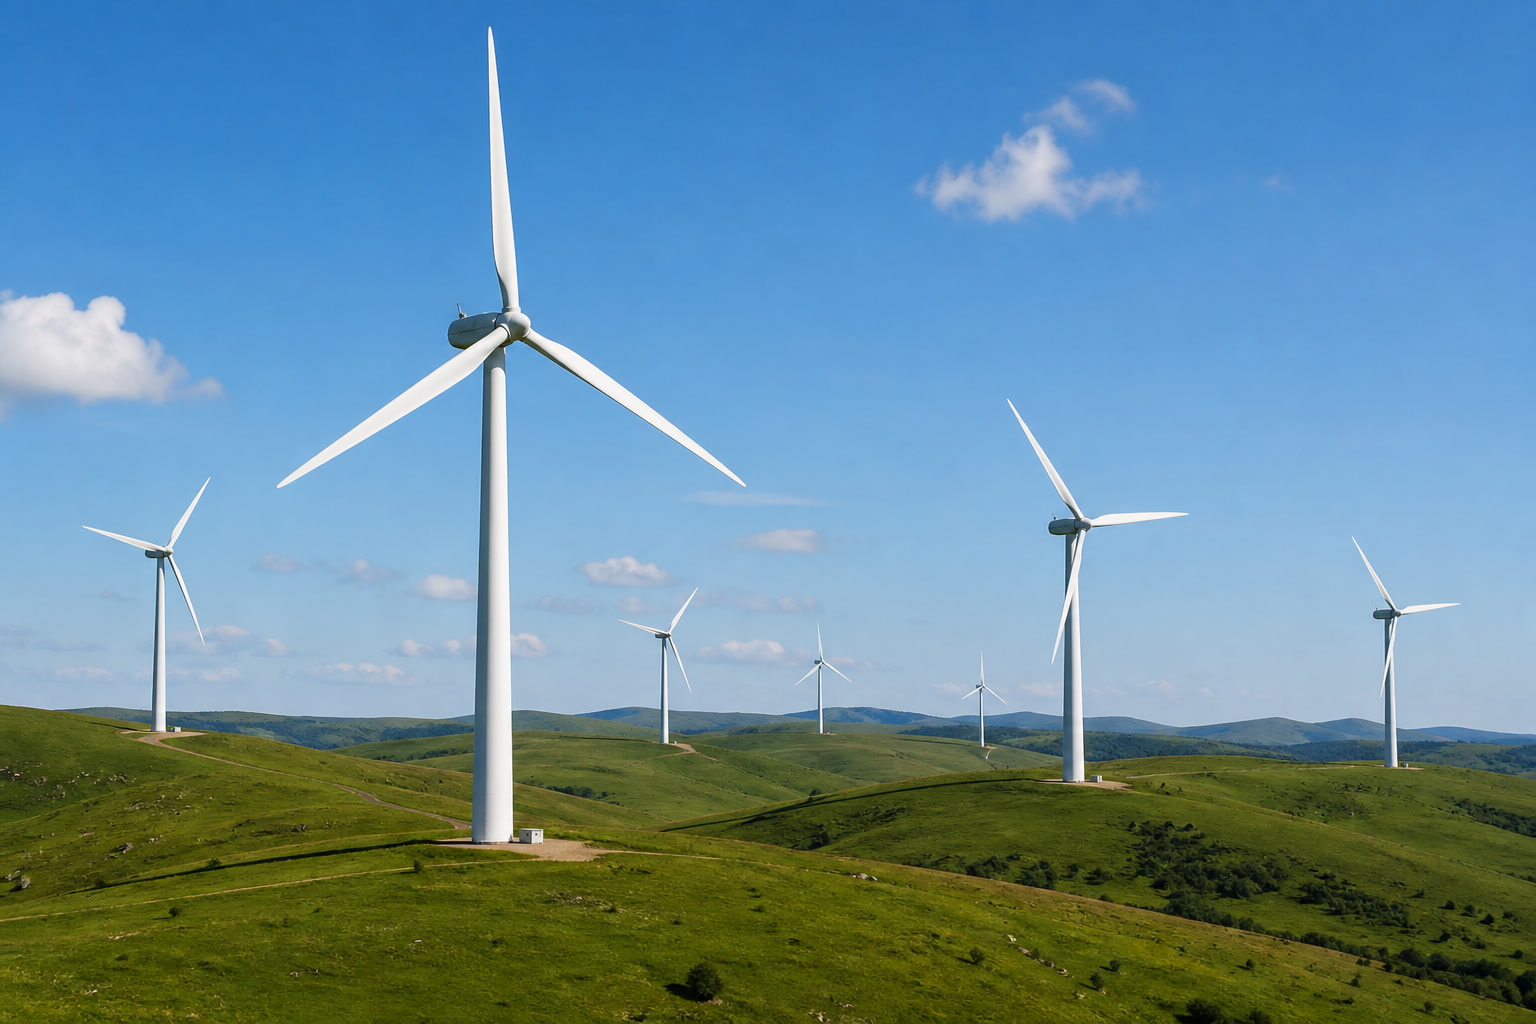
\includegraphics[width=0.58\linewidth]{images/book1/ai/g5-energy-windfarm.jpg}

{\small सड़क से ही दिख जाने वाली एक \omterm{def:g5:everyday-energy:energy}{ऊर्जा} शृंखला: चलती \omterm{def:g2:air-around-us:air}{हवा} पंख घुमाती है, और टरबाइन तारों में विद्युत \omterm{def:g5:everyday-energy:energy}{ऊर्जा} भेज देते हैं।}
\end{omfigure}

\section{मेज़ के सिरहाने बैठा सूर्य}

\begin{example}[लगभग हर शृंखला सूर्य से शुरू होती है]\label{ex:g5:everyday-energy:sun}
ज़्यादातर शृंखलाओं का पीछा उलटी दिशा में करो, तो तुम सूर्य तक पहुँच
जाते हो। नाश्ता? उसे पौधों ने सूर्य का \omterm{def:g1:light-and-shadows:source}{प्रकाश} पकड़कर उगाया; तुम्हारा
दलिया डिब्बाबंद धूप है। \omterm{def:g2:air-around-us:wind}{पवन}? सूर्य ज़मीनों को अलग-अलग ढंग से गरम करता
है, और हिलती हुई \omterm{def:g2:air-around-us:air}{हवा} ही \omterm{def:g2:air-around-us:wind}{पवन} है --- यानी पालवाली नावें भी धूप से चलती
हैं। लकड़ी? पेड़ों की सँभाली हुई धूप। बाँध का ऊँचाई वाला पानी? उसे
सूर्य ने उठाया: उसने समुद्र को \omterm{def:g2:ice-water-steam:evapcond}{वाष्पित} किया, और वह वाष्प पहाड़ों पर
बरस पड़ी। सौर पट्टिकाएँ तो बस बिचौलियों को छोड़ देती हैं।
\end{example}

\begin{omfigure}
\begin{tikzpicture}[scale=0.85]
  \fill[omThm] (0.9,3.2) circle (0.45);
  \foreach \a in {0,30,...,330} {
    \draw[omThm] (0.9,3.2) ++(\a:0.62) -- ++(\a:0.26);
  }
  \node[below, font=\small] at (0.9,2.5) {सूर्य};
  \node[draw, thick, omMeth, font=\small] (p) at (4.3,3.2) {पौधे};
  \node[draw, thick, omDef, font=\small] (f) at (7.2,3.2) {भोजन};
  \node[draw, thick, omMeth, font=\small] (m) at (9.9,3.2) {माँसपेशियाँ};
  \node[draw, thick, omMeth, font=\small] (w) at (4.3,1.4)
    {गरम होकर हिलती हवा};
  \node[draw, thick, omDef, font=\small] (v) at (8.3,1.4)
    {पवन और पाल};
  \draw[-Stealth, very thick] (1.6,3.2) -- (p);
  \draw[-Stealth, very thick] (p) -- (f);
  \draw[-Stealth, very thick] (f) -- (m);
  \draw[-Stealth, very thick] (1.35,2.75) -- (w);
  \draw[-Stealth, very thick] (w) -- (v);
\end{tikzpicture}

{\small अपने स्रोत तक पीछे ले जाई गई दो शृंखलाएँ: नाश्ता और \omterm{def:g2:air-around-us:wind}{पवन},
दोनों सूर्य से शुरू होते हैं।}
\end{omfigure}

\begin{remark}[एक शब्द, जिसे हम और पैना करेंगे]\label{rem:g5:everyday-energy:promise}
अभी के लिए \omterm{def:g5:everyday-energy:energy}{ऊर्जा} एक अच्छी तरह सुनाई गई कहानी है: भंडार, रूप,
शृंखलाएँ। क्या उसे \emph{मापा} भी जा सकता है, जैसे लंबाई मीटरों में
और \omterm{def:g3:measuring-mass:mass}{द्रव्यमान} ग्रामों में? जा सकता है --- \omterm{def:g5:everyday-energy:energy}{ऊर्जा} का अपना \omterm{def:g2:measuring-length:measure}{मात्रक} है और
अपना पक्का हिसाब-किताब, और वे इसी पुस्तक में आगे आते हैं, जब तुम चाल
और \omterm{def:g2:pushes-and-pulls:force}{बल} से ठीक से मिल चुके होगे। इस साल तुम जिन शृंखलाओं का पीछा कर रहे
हो वे नक़्शा हैं; संख्याएँ आकर उसी पर बस जाएँगी।
\end{remark}

\section{अभ्यास}

\begin{exercise}[$\star$]\label{exo:g5:everyday-energy:1}
इस अध्याय के शब्दों में \omterm{def:g5:everyday-energy:energy}{ऊर्जा} क्या है? ऐसी चार चीज़ें बताओ जो उसके
बिना हो ही नहीं सकतीं।
\end{exercise}

\begin{exercise}[$\star$]\label{exo:g5:everyday-energy:2}
भंडार ढूँढ़ो: दौड़ता चाबी वाला चूहा; \ साइकिल चलाता कोई व्यक्ति; \
अलाव; \ पालवाली नाव; \ टॉर्च।
\end{exercise}

\begin{exercise}[$\star$]\label{exo:g5:everyday-energy:3}
\omterm{def:g5:everyday-energy:energy}{ऊर्जा} के पाँच रूप बताओ, और हर एक का एक उदाहरण अपने दिन में से।
\end{exercise}

\begin{exercise}[$\star$]\label{exo:g5:everyday-energy:4}
\cref{met:g5:everyday-energy:read} की तरह टोस्टर की \omterm{def:g5:everyday-energy:energy}{ऊर्जा} शृंखला का
पीछा करो: भंडार, रूपांतरक, बाहर निकलने वाले रूप।
\end{exercise}

\begin{exercise}[$\star$]\label{exo:g5:everyday-energy:5}
बाँध की झील से लेकर आज रात तुम्हारे पढ़ने वाले लैंप तक की शृंखला का
पीछा करो।
\end{exercise}

\begin{exercise}[$\star$]\label{exo:g5:everyday-energy:6}
कोई फ़ोन ``मर जाता'' है। असल में ख़त्म क्या हुआ? शृंखला वाली
प्रतिज्ञप्ति के अनुसार वह \omterm{def:g5:everyday-energy:energy}{ऊर्जा} गई कहाँ?
\end{exercise}

\begin{exercise}[$\star$]\label{exo:g5:everyday-energy:7}
काम करते समय लैपटॉप नीचे से गरम क्यों हो जाता है? शृंखला की कौन-सी
कड़ी ख़ुद को दिखा रही है?
\end{exercise}

\begin{exercise}[$\star$]\label{exo:g5:everyday-energy:8}
शृंखला का क़दम-दर-क़दम उलटा पीछा करके दिखाओ कि पालवाली नाव धूप से
चलती है।
\end{exercise}

\begin{exercise}[$\star\star$]\label{exo:g5:everyday-energy:9}
एक आविष्कारक ऐसे लैंप की घोषणा करता है जिसे ``न \omterm{def:g3:first-electric-circuit:battery}{बैटरी} चाहिए, न प्लग,
न ईंधन --- वह बस हमेशा जलता रहता है''। यह घोषणा
\cref{rem:g5:everyday-energy:nofree} के किस सबक़ को ठेंगा दिखाती है?
आविष्कारक से सबसे पहले कौन-सा सवाल पूछना चाहिए?
\end{exercise}

\begin{exercise}[$\star\star$]\label{exo:g5:everyday-energy:10}
कंधे की ऊँचाई से गिराई गई रबर की गेंद हर बार पहले से नीची उछलती है
और आख़िर में चुपचाप पड़ी रह जाती है। लियो कहता है, ``उसकी \omterm{def:g5:everyday-energy:energy}{ऊर्जा} नष्ट
हो गई।'' \cref{prop:g5:everyday-energy:chain} की मदद से कहानी का
इससे बेहतर अंत सुझाओ --- उछलने की \omterm{def:g5:everyday-energy:energy}{ऊर्जा} आख़िर किस रूप में फिसल गई?
\end{exercise}

\begin{exercise}[$\star\star$]\label{exo:g5:everyday-energy:11}
कुछ घर छत पर लगी काली पट्टिकाओं में पानी गरम करते हैं; कुछ धूप और
मुड़े हुए दर्पणों से खाना पकाते हैं; और सौर सेल दिन के उजाले से बिजली
बनाते हैं। \cref{ex:g5:everyday-energy:sun} वाला वाक्य ``सौर
पट्टिकाएँ तो बस बिचौलियों को छोड़ देती हैं'' समझाओ: सूर्य और लकड़ी की
आग की गरमी के बीच कौन-से बिचौलिये खड़े हैं?
\end{exercise}
